\documentclass{article}

\usepackage[russian]{babel}
\usepackage{amsmath}
\usepackage{hyperref}
\usepackage{graphicx}
\usepackage{mathtools}


\usepackage[dvipsnames]{xcolor}

\title{Differential Equations Computational Practicum}
\date{2019-11-14}
\author{Timur Gainullin}


\begin{document}
  \pagenumbering{gobble}
  \maketitle

  \newpage
  \pagenumbering{arabic}



  \section{Introduction}

  Given the initial value problem:
  \[
    \begin{dcases}
      y' = 1 + 2y / x\\
      y(1) = 2\\
      x \in (1, 10)
    \end{dcases}
  \]

  Needed to solve it analytically and using 3 numerical methods. Solutions should be analyzed and compared to each other. To provide data visualization I chose JavaFX and used OOP-design in code structure. Repository is available
  \href{https://github.com/Tumypmyp/DE_Practicum}{\color{blue}{\underline{here}}}. But first, let us find the exact solution for this equation.


  \section{Analytical solution}

  $$y' = 1 + \frac{2y}{x}$$

  $$y' - \frac{2y}{x} = 1$$

  A nonhomogeneous equation of form y' + f(x)y = g(x) and can be
  solved using the integrating factor:

  $$\mu(x) = e^{\int{\frac{-2}{x} \partial x}} = x^{-2}$$
  $$\frac{\frac{\partial y}{\partial x}}{x^2} - \frac{2y}{x^3} = \frac{1}{x^2}$$
  $$\frac{\frac{\partial y}{\partial x}}{x^2} - \frac{\partial}{\partial x}\left(\frac{1}{x^2}\right)y = \frac{1}{x^2}$$

  Apply the reverse product rule:
  $$\frac{\partial}{\partial x}\left(\frac{y}{x^2}\right) = \frac{1}{x^2}$$

  Integrate both sides with respect to $x$:
  $$\int{\frac{\partial}{\partial x}\left(\frac{y}{x^2}\right)}\partial x = \int{\frac{1}{x^2}}\partial x$$
  $$ \frac{y}{x^2} = -\frac{1}{x} + c_1$$
  $$y = x(c_1x - 1)$$

  Using $y(1) = 2$:

  $$2 = c_1 - 1$$
  $$c_1 = 3$$
  The solution is:
  $$y = x(3x - 1), \quad x \neq 0$$

  \section{Numerical solutions}

  \subsection{Application}
  There is some screenshots of application:\\ \\
  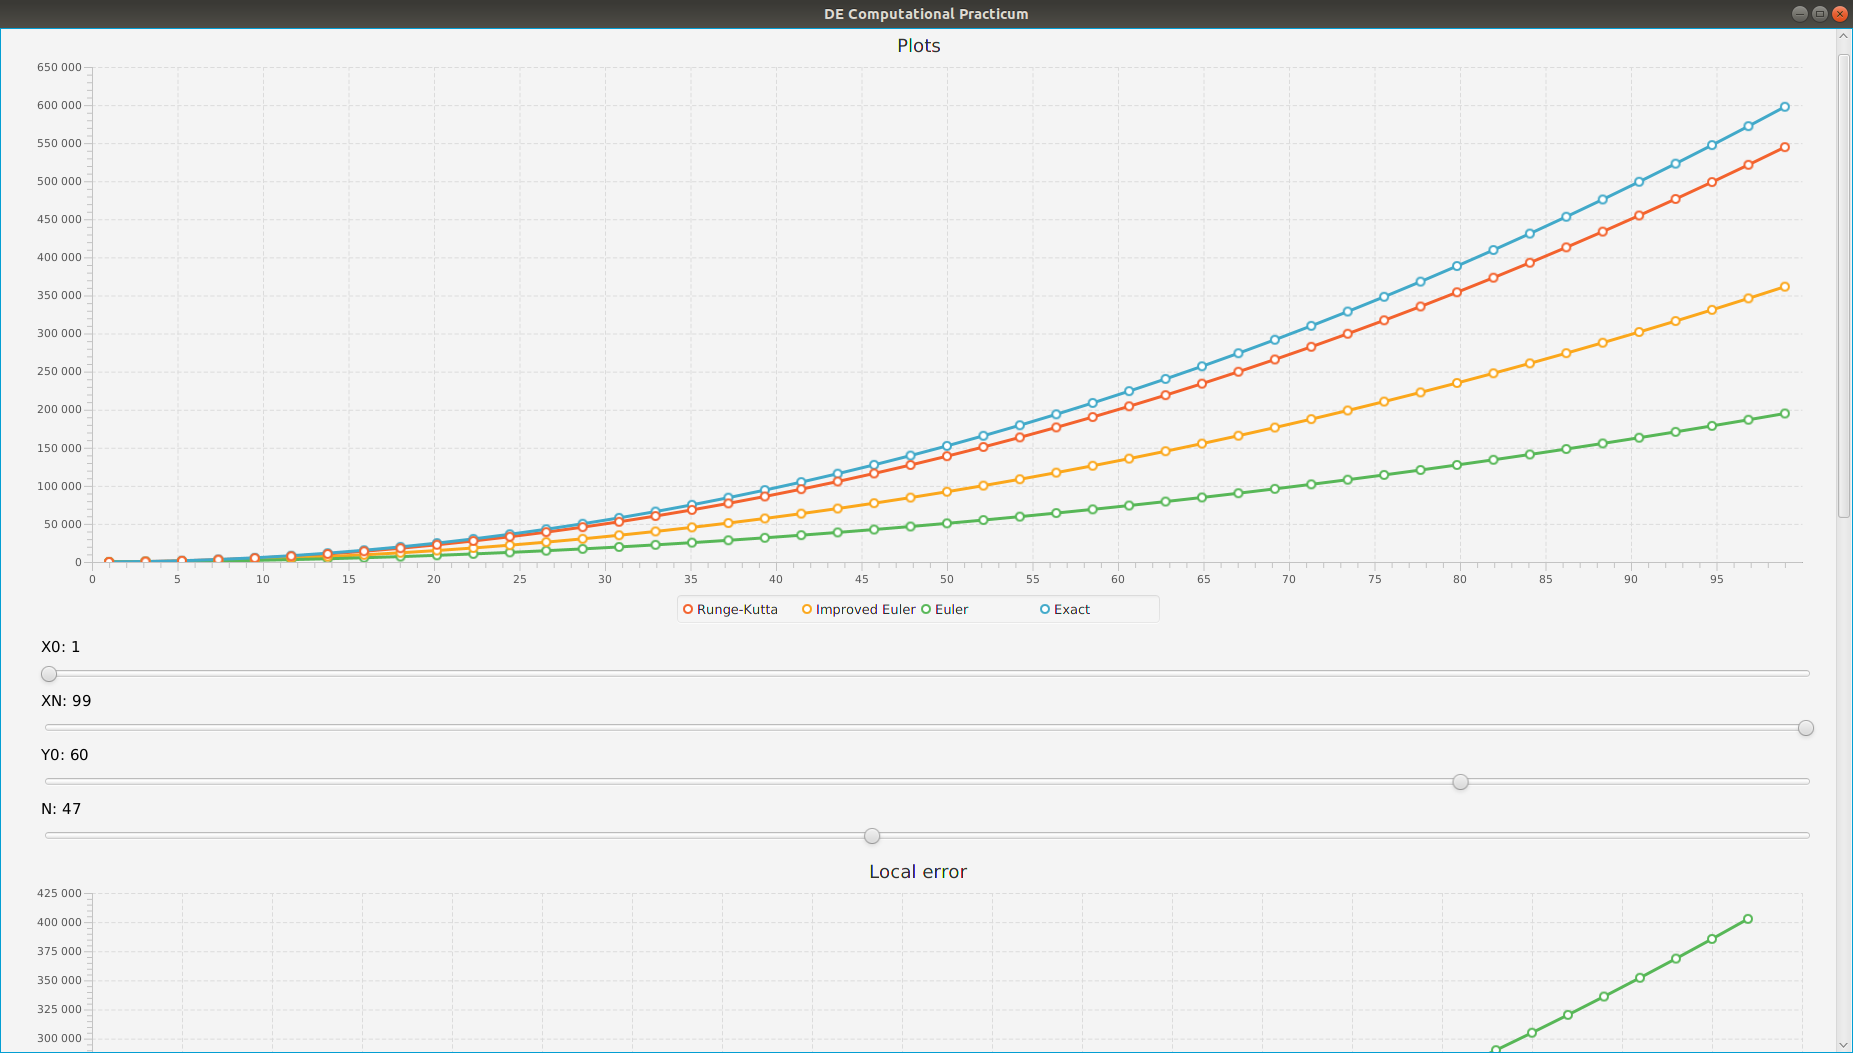
\includegraphics[scale=0.2]{Plots.png} \\
  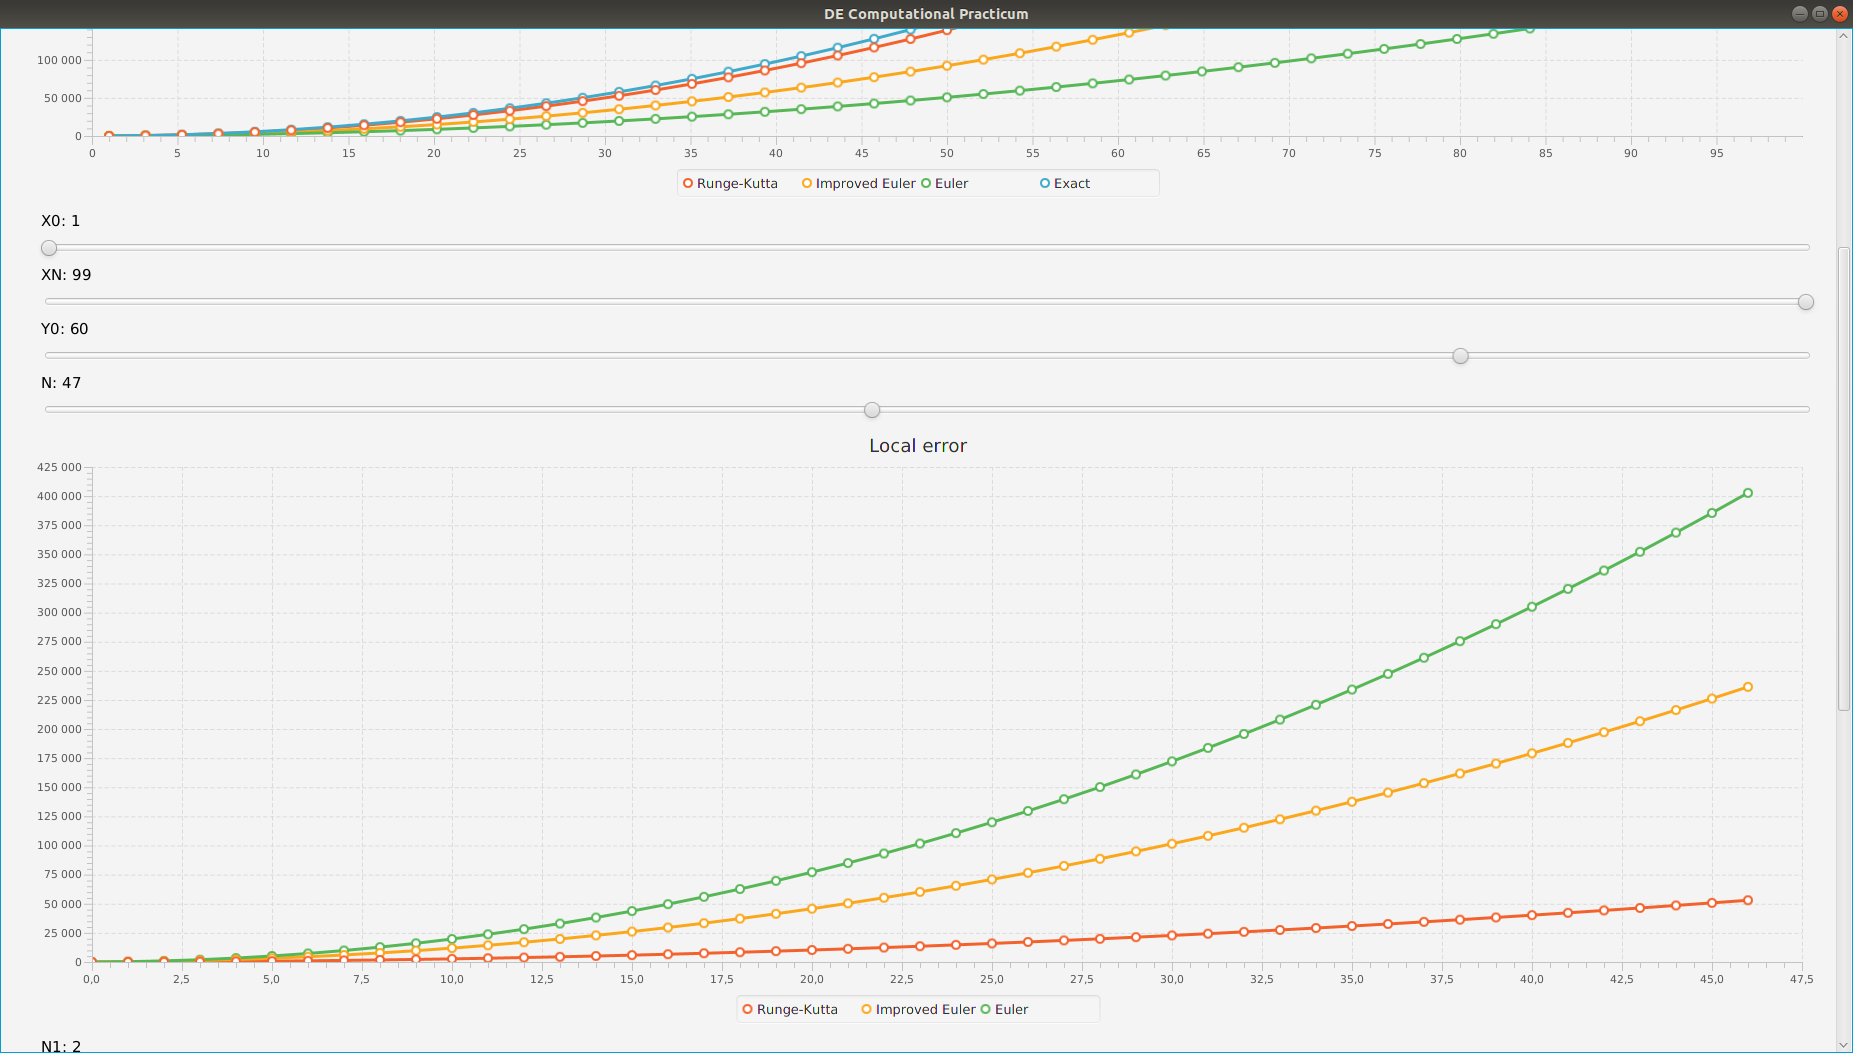
\includegraphics[scale=0.2]{LocalErrors.png} \\
  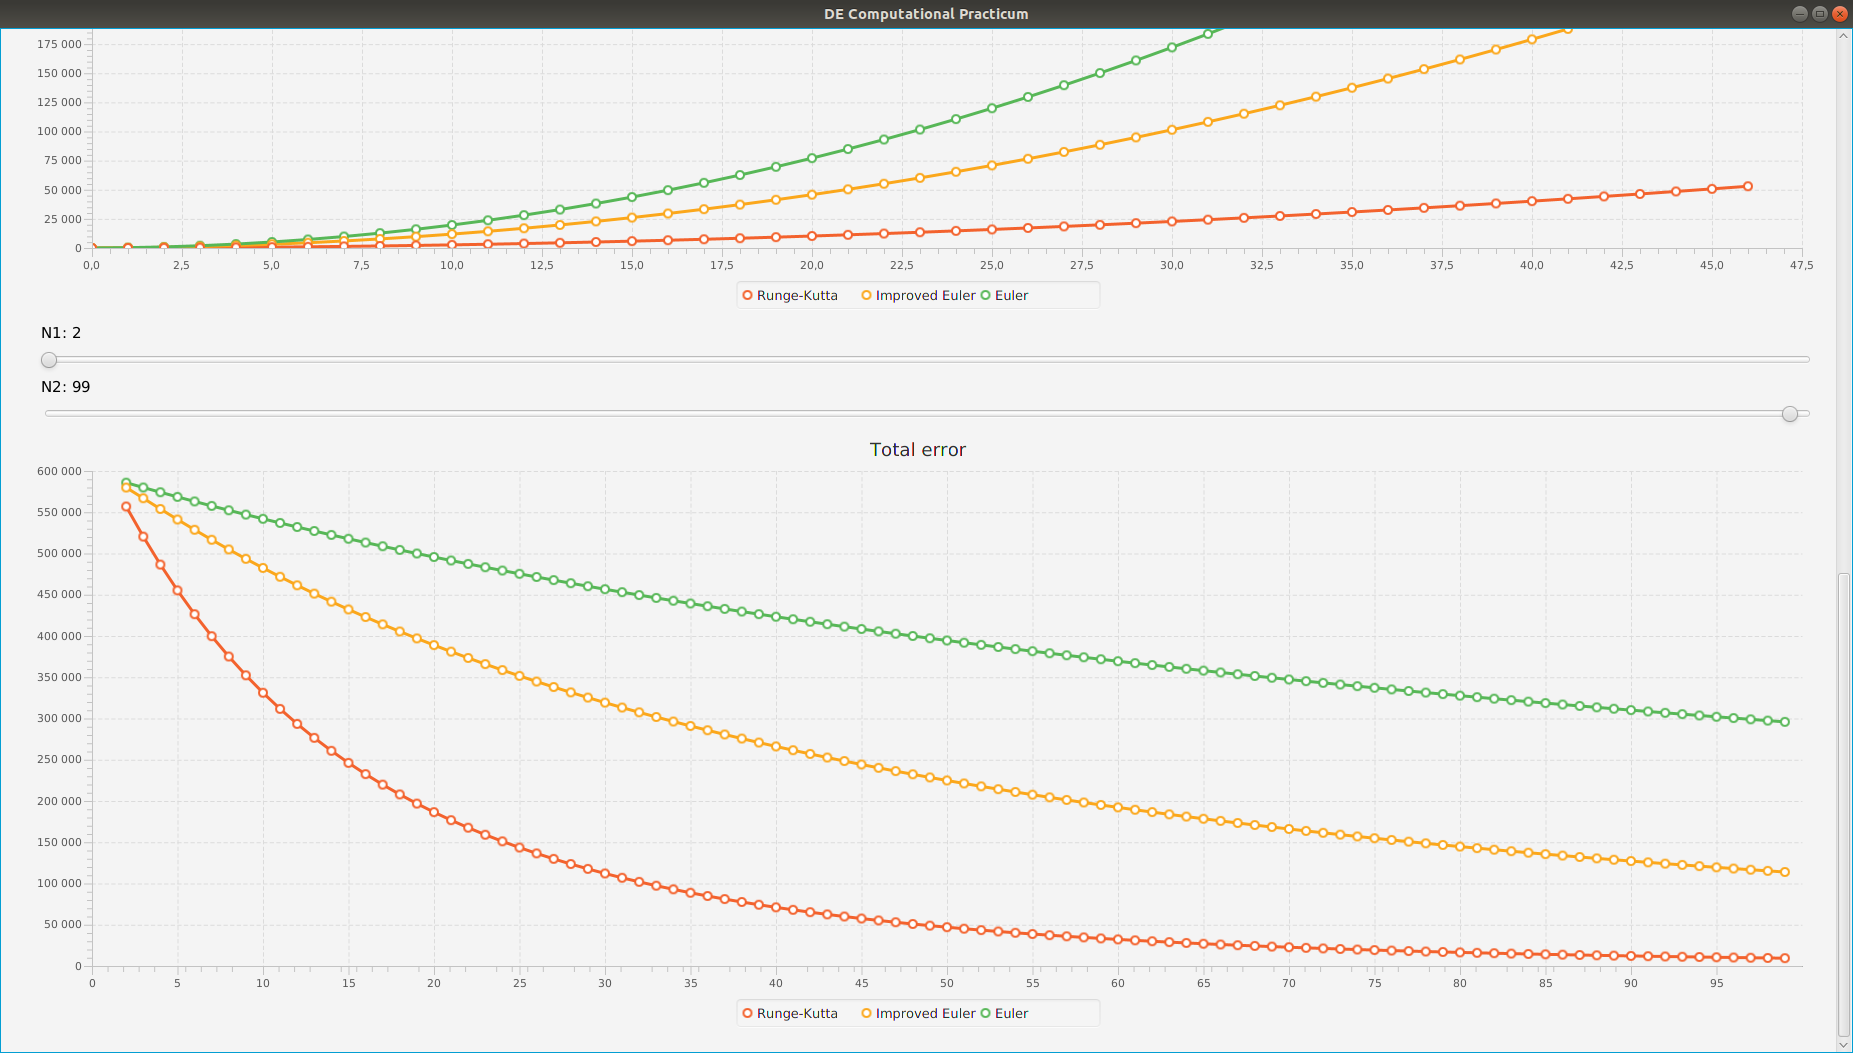
\includegraphics[scale=0.2]{TotalErrors.png}

  \subsection{UML-diagram}
  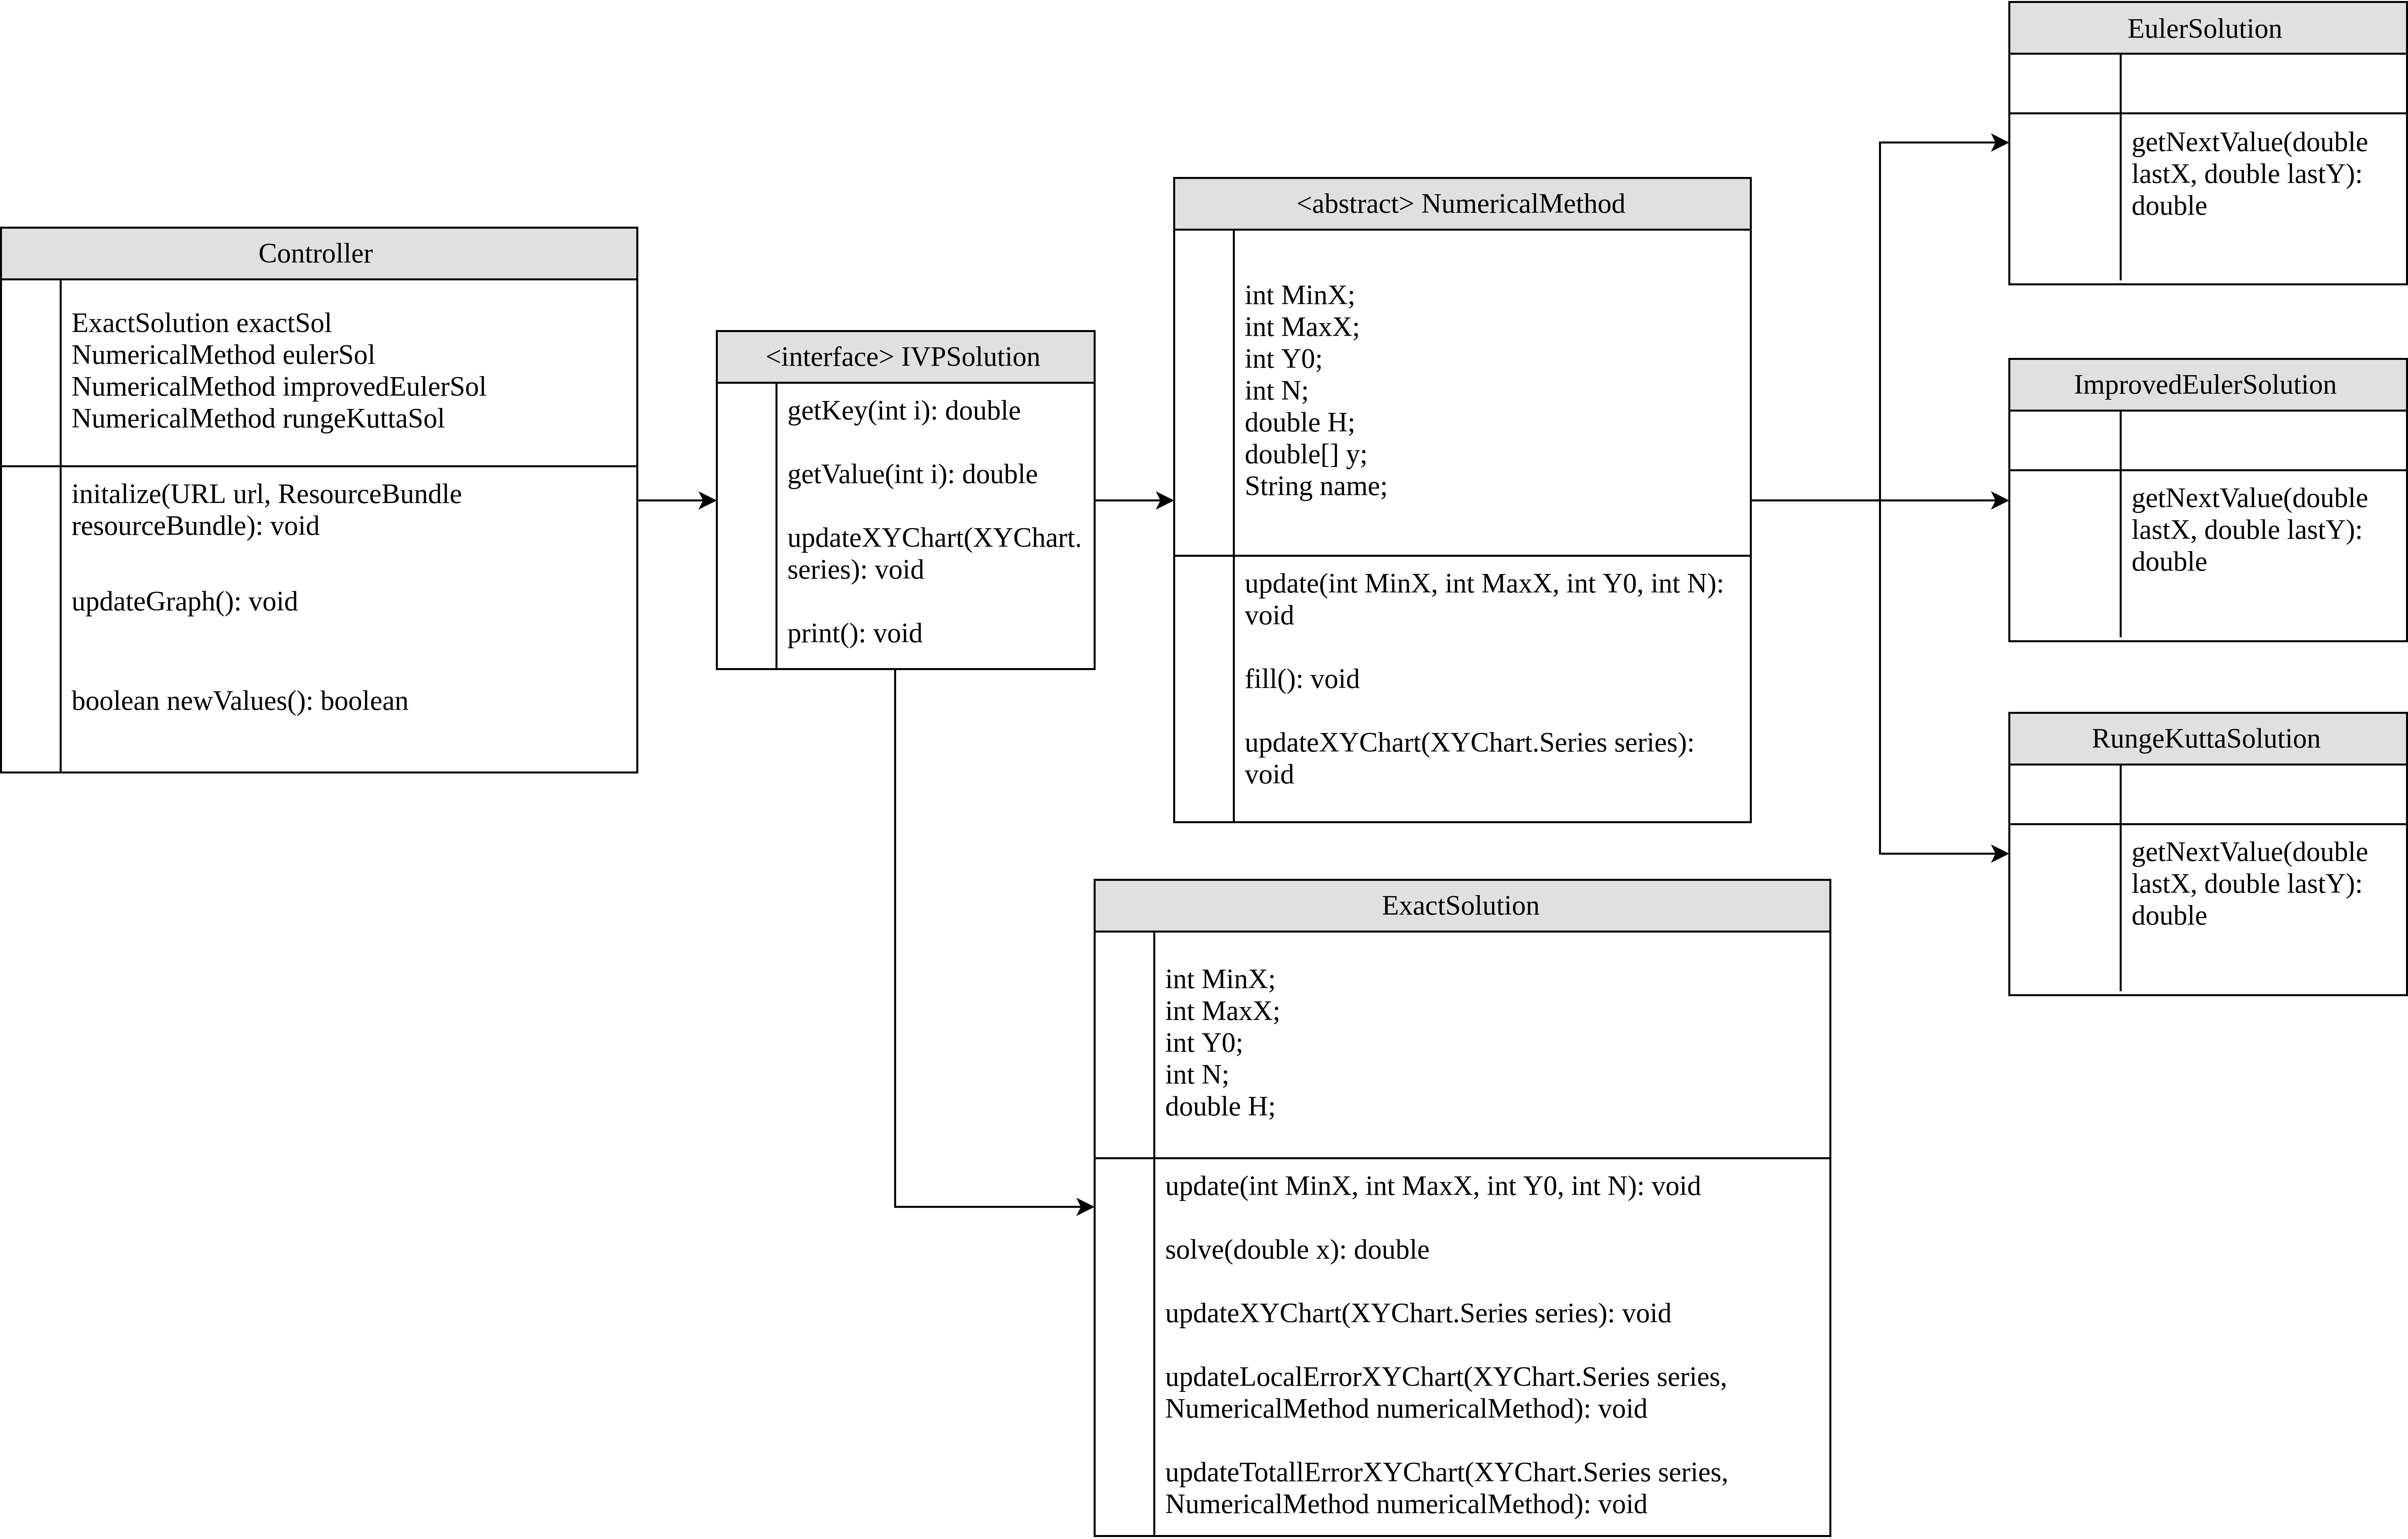
\includegraphics[scale=0.5]{UML.png}

  \subsection{Code}
  To avoid same code for different \texttt{NumericalMethod}s when we need to calculate local and total errors
  I wrote function that updates this graph in \texttt{ExactSolution} class. This is code I got with function
  that just updates solution for comparation:


  \begin{verbatim}
    public void updateXYChart(XYChart.Series series) {
    series.getData().clear();
    for (int i = 0; i < N; ++i) {
    series.getData().add(new XYChart.Data(getKey(i), getValue(i)));
    }
    }

    public void updateLocalErrorXYChart(XYChart.Series series,
    NumericalMethod numericalMethod) {
    series.getData().clear();
    for (int i = 0; i < N; ++i) {
    series.getData().add(new XYChart.Data(i, getValue(i)
    - numericalMethod.getValue(i)));
    }
    }

  \end{verbatim}

  The \texttt{NumericalMethod} unites all 3 methods because they are exactly the same
  but with different formulas to get next $y_i$. There is part of the abstract class that shows it:

  \begin{verbatim}
    private void fill() {
    y = new double[N];
    y[0] = Y0;
    for (int i = 1; i < N; i++) {
    y[i] = getNextValue(getKey(i - 1), y[i - 1]);
    }
    }

    abstract double getNextValue(double lastX, double lastY);
  \end{verbatim}

  \subsection{Conclution}

  That way we can see how Eule's, improved Euler's and Runge-Kutta methods works compare to each other
  and Exact solution on given IVP.

\end{document}
